
{\rmfamily
\vspace{-2em}
This work was previously published in ACM SIGCHI 2016 \cite{ka} and has been adapted for this document.
\vspace{2em}
}

%Effectively understanding online information has become increasingly challenging for individuals as the amount of information available for learning and decision making grows. One promising approach is to use crowds to filter, parse, and synthesize information in a distributed manner. However, making sense of online information is a highly complex and interdependent cognitive task, making it difficult to distribute to crowd workers each with only a local view. We present a crowd-powered information synthesis approach which addresses these challenges, and introduce a set of design patterns for such ``big little thinking'', including supporting global context, leveraging worker choice, and delaying structuring, that may also be useful for other types of crowds and tasks. We evaluate a system embodying the approach against top information sources on the web, finding that its outputs are perceived favorably compared to top Google results for a given question.%

%Crowdsourcing offers a powerful new paradigm for online work. However, real world tasks are often interdependent, preventing them from being easily decomposed and distributed. While existing crowdsourcing approaches offer solutions to task decomposition, no systems offer a distributed solution to the context required to manage the task. In this paper, we explore crowdsourcing one of these complex, interdependent tasks: information synthesis. We introduce a system that accomplishes this feat, known as the Knowledge Accelerator (KA), and introduce a set of design patterns for complex, interdependent crowdsourcing. These patterns, which may also be useful for other types of crowds and tasks, include supporting global context, leveraging worker choice, and developing distributions. We evaluate this system, and find overall that its output is rated higher than the top five Google results for information synthesis questions posed to it. 


Crowdsourcing offers a powerful new paradigm for online work. However, real world tasks are often interdependent, requiring a big picture view of the difference pieces involved. Existing crowdsourcing approaches that support such tasks --- ranging from Wikipedia to flash teams --- are bottlenecked by relying on a small number of individuals to maintain the big picture. In this paper, we explore the idea that a computational system can scaffold an emerging interdependent, big picture view entirely through the small contributions of individuals, each of whom sees only a part of the whole. To investigate the viability, strengths, and weaknesses of this approach we instantiate the idea in a prototype system for accomplishing distributed information synthesis and evaluate its output across a variety of topics.  We also contribute a set of design patterns that may be informative for other systems aimed at supporting big picture thinking in small pieces.\cite{ka}


\section{Introduction}

Crowdsourcing is a powerful mechanism for accomplishing work online. By decomposing and distributing the cognitive work of an individual, crowdsourcing can provide a larger pool of resources more quickly and with lower transaction costs than through traditional work. A common emerging theme is that the more a task can be split, simplified, and distributed into smaller subtasks, and the lower the cost of accepting and completing a task, the larger the pool of workers accessible who can complete it anywhere at anytime \cite{kittur2013future}. For example, microtask markets such as Amazon Mechanical Turk (AMT) enable hundreds of thousands of workers from across the globe to be recruited within seconds \cite{Bernstein:2011:CTS:2047196.2047201}.
 
However, much work in the real world is not amenable to crowdsourcing because of the difficulty in decomposing tasks into small, independent units. As noted by many researchers \cite{bernstein2010soylent, kittur2011crowdforge, little2010turkit, Luther:2013:RLO:2441776.2441891}, decomposing tasks --- ranging from writing an article to creating an animated film --- often results in pieces that have complex dependencies on each other. Take for example the goal of writing an article that synthesizes information on the web about a given topic (e.g., growing better tomatoes). Coming up with a coherent and comprehensive set of topics (e.g., soil, sunlight, watering, pruning) is challenging without a global view of the data. The need for coherence extends throughout the fractal nature of the article: each section, paragraph, and sentence must have a proper transition and flow. Supporting such work requires having a big picture view of different pieces at different scales and ensuring they all fit together.

Accomplishing big picture thinking through small tasks is challenging because it means that each person can only have a limited view of the bigger picture. As a result, many of the applications of crowdsourcing have been limited to simple tasks such as image labeling where each piece can be decomposed and processed independently. Those approaches that do crowdsource tasks requiring big picture thinking --- such as volunteer communities such as Wikipedia, open source software, or paid crowd work approaches such as flash teams \cite{retelny2014expert} or Turkomatic \cite{kulkarni2012collaboratively} --- have relied on a heavily invested contributor such as a moderator or an experienced contributor to maintain the big picture. For example, in Wikipedia a large proportion of the work is done by a small group of heavily invested editors \cite{kittur2007he}, and the quality of an article is critically dependent on there being a small number of core editors who create and maintain a big picture structure for more peripheral members to contribute effectively \cite{kittur2008harnessing}. 

A reliance on a single or a small number of individuals to maintain the big picture creates a bottleneck on the size and complexity of task amenable to crowdsourcing, and also results in brittleness: if the person maintaining the big picture leaves, it can cause serious problems for the group task. This is a real problem that online production communities are facing; for example, Wikipedia has identified as a key challenge that it is losing core editors faster than it can attract and grow new ones \cite{suh2009singularity}. As these core editors are disproportionately responsible for not only producing content but also for creating a structure for peripheral contributions, their departure is particularly difficult to handle. Taking a step towards enabling the production of complex artifacts through many contributors making small contributions might thus have implications in reducing individual bottlenecks in microtask markets and beyond.
 
% In this paper we investigate whether a big picture view can be supported entirely through small distributed tasks without the bottleneck of a single individual maintaining global coherence. Specifically, we investigate whether a computational system can act as a scaffold by providing the appropriate context and coordination to individual crowd workers. This would enable them to collectively generate a big picture view and enforce the multi-level interdependent constraints it entails, even though each individual sees only a small part of the whole.

Our main contribution in this paper is the idea that a computational system can scaffold an emerging interdependent, big picture view entirely through small contributions of individuals, each of whom sees only a part of the whole. To investigate this idea we instantiate it in a working software system to explore the viability, strengths, and weaknesses of the approach, and evaluate the output of the system across a variety of topics. Finally, we also contribute a set of design patterns that may be informative for other systems aimed at supporting big picture thinking in small packages.

\begin{figure*}
    \centering
    \frame{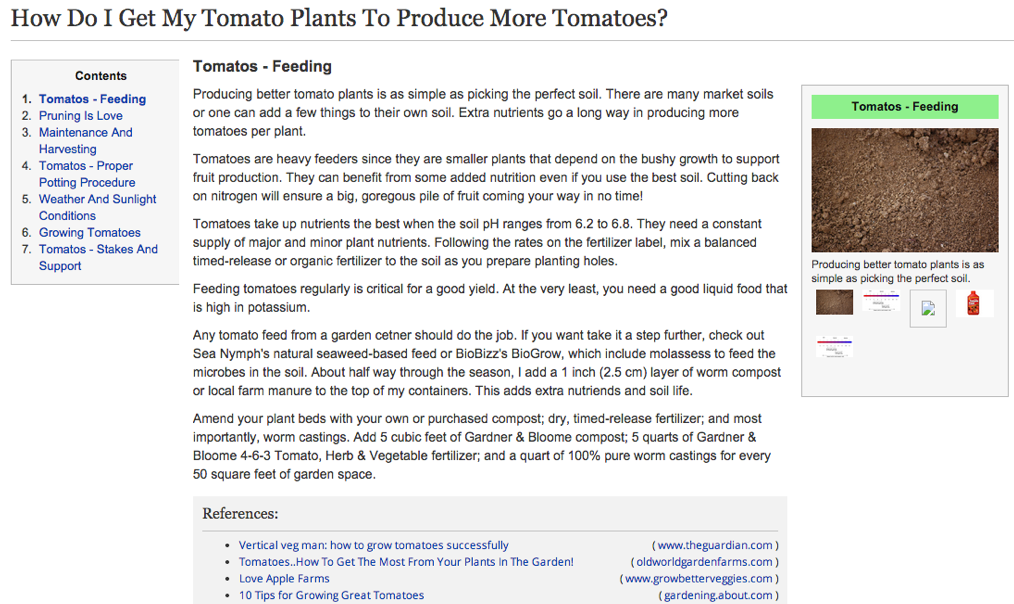
\includegraphics[width=1\columnwidth]{Chapters/KA/final_answer}}
    \caption{The final output of the Knowledge Accelerator system.}
    \label{fig:final_answer}
\end{figure*}
%\michelle{does the description of the task warrant its' own section? not sure... you've probably debated this already and decided this is the best approach, but it seems like at this point, you could skip to the contributions paragraph without needing the info about the task and put a section about the specific situation after?}



\subsection{System Overview}
The ``Knowledge Accelerator'' (KA) is a prototype system which uses crowd workers each contributing small amounts of effort to synthesize online information for complex and/or open-ended questions. The KA system starts with a given question (such as ``How do I deal with the arthritis in my knee as a 28 year old'') and crowdsources the generation of a coherent article that synthesizes different sources, viewpoints, and topics found online relevant to answering the question. Critically, the KA system accomplishes this process without a core overseer or moderator. 

As the goal of the system was to probe how to accomplish a complex information synthesis task entirely through relatively small contributions, we limited our maximum task payment to \$1 US, aimed at incentivizing a target task time of approximately 5-10 minutes. We chose this approach because a fixed payment amount matches the structure of many microtask crowdsourcing markets (e.g., versus a fixed time period of 10 minutes). While some crowdsourcing markets (such as UpWork or eLance) do support hourly rates and fixed time periods, the double-sided transaction (or ``handshake'') costs in which employers and workers vet each other in such markets would constitute a substantial fraction of the working time we target, and the time scale of projects in such markets (typically measured in hours) do not match well with the time scale of the projects we target here (i.e., minutes).\footnote{One concern could be that \$1 could motivate different amounts of effort across different countries. For all tasks other than sourcing and clipping we limited the pool of workers for our tasks to U.S. workers to control for cross-country currency differences. For sourcing and clipping workers U.S. workers spent an average of 9.72 minutes and 6.89 minutes respectively, while non-U.S. workers spent 8.65 minutes and 8.36, which were not significantly different.} 

An example of the output of the system for the target question ``How do I get my tomato plants to produce more tomatoes?'' can be found in Figure~\ref{fig:final_answer}. To produce this output workers find high value sources from the web (e.g., gardening.about.com), extract the useful and relevant clips of information from them, cluster these clips across sources into commonly discussed topics (e.g., feeding or pruning), and generate an article for each topic that synthesizes the relevant clips into coherent chunks of information while reducing redundancies (e.g., if several sources all mention soil pH range, the article should not include that information multiple times). Workers also find relevant multimedia images and video to illustrate each chunk. Information sources used in the creation of the article are referenced in the final output, and the article is organized by subtopics with the most diverse set of references first (See Figure \ref{fig:process} for the KA process overview). 

Our primary contribution in addressing this task is to further our theoretical understanding of the mechanisms and limitations of accomplishing big picture thinking in small pieces, which may have implications for crowdsourcing systems that aim to do complex cognitive tasks including microtask crowdsourcing \cite{kittur2013future}, peer production communities \cite{kittur2008harnessing}, friendsourcing \cite{bernstein2010personalization}, and selfsourcing \cite{teevan2014selfsourcing}. However, addressing this task may also have intrinsic utility in paving the road for crowdsourced systems that can synthesize complex information from a variety of sources on demand. Such systems may be especially useful for topics not be covered by traditional online sources; examples include low frequency or highly personalized search queries (such as looking for information on a particular medical condition given the person's context including age or other symptoms), topics whose sources are highly unstructured and distributed (such as advice giving on discussion forums), or for information that is inside an organization's firewall (such as for a company's IT support sessions). 

%One interesting example we found was for automative diagnostics questions (e.g., ``2003 Dodge Durango has an OBD-II error code of P440. How do I fix it''), where workers synthesized many valuable but unstructured sources of information in car enthusiast forums into a coherent digest. Compared to two commercially available expert-generated databases we found that the system's topics not only covered the solutions but also added ``long tail'' solutions (such as identifying that if the truck was stored in a barn the code is often triggered by mice nesting in the undercarriage for heat) that were considered valuable additions by automotive experts. In the Evaluation section we compare the system's output to a variety of online sources ranging from expert-generated high-traffic sources (e.g., The CDC website) to unstructured user generated sources (e.g., car enthusiast forums).

Below we discuss the challenges involved in developing the system, particularly focusing on issues central to supporting big picture thinking with workers each seeing only a small part of the whole. We first discuss related work, describe the system architecture, then evaluate the utility of the system’s output versus top online sources across a variety of topics.


%%\subsection{Task Selection}

%%To explore this question we set as our goal creating a Wikipedia-like article on an arbitrary topic with no single task paying more than \$1. Creating an encyclopedia-like digest for a target topic (such as how to fix a boiler or what to do about retirement) is an easy to understand task that nonetheless involves several complex and interdependent challenges, including determining a good structure for the article and synthesizing information for different sources into a coherent whole. As we discuss later, the \$1 limit forces the system to avoid bottlenecks where individuals are doing disproportionately large amounts of work.%\niki{I'm not sure what the purpose of this is.  Put here it seems to imply that you could get more value for a dollar by using other workers, but then provides evidence that actually you don't. If it's about addressing the concern that a dollar buys different amounts of work that seems important to have but doesn't seem to fit here; maybe change this to a footnote in the task selection section instead?} 
%%\footnote{One concern could be that \$1 could motivate different amounts of effort across different countries. For all tasks other than sourcing and clipping we limited the pool of workers for our tasks to U.S. workers to control for cross-country currency differences. For sourcing and clipping workers U.S. workers spent an average of 9.72 minutes and 6.89 minutes respectively, while non-U.S. workers spent 8.65 minutes and 8.36, which were not significantly different.} By doing so we aim to further our theoretical understanding of the mechanisms and limitations of accomplishing big picture thinking in small pieces, which may have implications for crowdsourcing systems that aim to do complex cognitive tasks including microtask crowdsourcing \cite{kittur2013future}, peer production communities \cite{kittur2008harnessing}, friendsourcing \cite{bernstein2010personalization}, and selfsourcing \cite{teevan2014selfsourcing}. 


% \jieun {I commented our this sentence and rephrased the previous sentence: Workers identified many valuable but unstructured \jieun{, dialog oriented} sources of information in car enthusiast forums, which the system synthesized into a coherent digest.

\section{Related Work}

\subsection{Crowdwork Complex Cognition and Workflow}

While most crowdsourcing approaches have focused on simple and/or independent tasks, there is a growing interest in crowdsourcing tasks that tap into complex and higher-order cognition \cite{kittur2013future}. Many of these fall into the class of decomposing cognitive processing in a structured way such that many workers can contribute \cite{ahmad2011jabberwocky, bernstein2010soylent, bigham2010vizwiz, kim2014crowdsourcing, kittur2011crowdforge, Kittur:2012:CVM:2145204.2145357, kulkarni2011turkomatic, lasecki2013warping, lasecki2013legion, little2010turkit}. Our work builds on this foundation by incorporating adaptive crowd workflows (e.g., TurKit, JabberWocky, CrowdWeaver), crowd-driven task generation (e.g, CrowdForge, Turkomatic), combining the outputs from decomposed tasks to create a global understanding (e.g., Cascade, Crowd Synthesis) and multi-stage crowd quality control process in which crowds can both generate new versions of output as well as vote on it (e.g., CrowdForge, Soylent, TurKit). However, we go beyond previous work in aiming to support a coherent big picture view while avoiding individual bottlenecks. Doing this is significantly more challenging than the tasks decomposed in prior research, requiring a search for structure during the sampling process, a reliance on novices to function with more context than they enter the task with, and a tight interdependence between each subtask such that any failures could negatively impact the value of the entire artifact. 

\vfill
\subsection{Information Synthesis}

Individual information synthesis is commonly associated with the process of sensemaking. Sensemaking can be characterized as the iterative process of building up a representation of an information space that is useful for achieving the user’s goal \cite{Russell:1993:CSS:169059.169209}. Theories of sensemaking provide a framework for characterizing and addressing the challenges faced by individuals and can point out leverage points for augmenting the process \cite{Russell:1993:CSS:169059.169209,dervin1983overview,klein2006making,karl1995sensemaking, gioia1991sensemaking,daft1984toward,milliken1990perceiving,pirolli1999information}. Generally, models agree that sensemaking is a dynamic and iterative process involving searching for information; filtering that information based on a user's goals and context; inducing a schema or structure from the information; and applying the schema to take action (e.g., writing a report, making a presentation).

A number of systems have been developed aimed at supporting these stages of sensemaking for an individual user \cite{baldonado1997sensemaker, dervin1992mind, dervin1998sense, Marchionini:2006:ESF:1121949.1121979, parameswaran2013datasift, law2011towards} or a group of users working together \cite{kittur2008harnessing, kittur2007he, morris2010wesearch, paul2009cosense, paul2010understanding,karl1995sensemaking}. However, prior research has focused almost exclusively on situations of integrated sensemaking in which individuals (even in groups) are heavily engaged in the entire sensemaking process. Instead, we aim to distribute the information synthesis process across many different individuals, each of whom may see only a limited view of the process.

Computational approaches to parts of the information synthesis process have also been investigated by many researchers. For example, Question Answering (QA) research addresses the methods and systems that automatically answering questions posted by human in natural language. The complex, interactive QA (ciQA) has been introduced at TREC 2006 and 2007 in addition to factoid and list QA \cite {dang2007overview}. However, automated QA approaches (and their crowd-based variants \cite{bernstein2012direct}) focuses on answering short, factual questions instead of the complex sensemaking processes we are interested in, where users build up rich mental landscapes of information.  Another approach is multi-document summarization \cite{barzilay1999information, goldstein2000multi, mani1997multi, mckeown1999towards}, which aims to use computational techniques to extract of information from multiple texts written for the same topic using feature based \cite{gupta2010survey}, cluster based \cite{jain1999data}, graph based \cite{erkan2004lexrank} and knowledge based methods \cite{hahn1999knowledge}. However, such approaches have limitations in dealing with complex yet short and sparse data that encountered on the web, and do not yet engage in the complex synthesis humans perform, which results in the cohesive and coherent output.

%Our approach addresses collaborative information foraging and sensemaking from a unique perspective of using distributed crowd workers alongside machine learning techniques. Compared to the above mentioned scenarios, crowd workers are characterized by easy accessibility, non-expert knowledge, and a limited amount of time to spend on one task \cite{kittur2013future}. Rather than having a completely algorithmic solution, we use a combination of human computation and automatic synthesis to produce a cohesive and coherent output.

\begin{figure*}
    \centering
    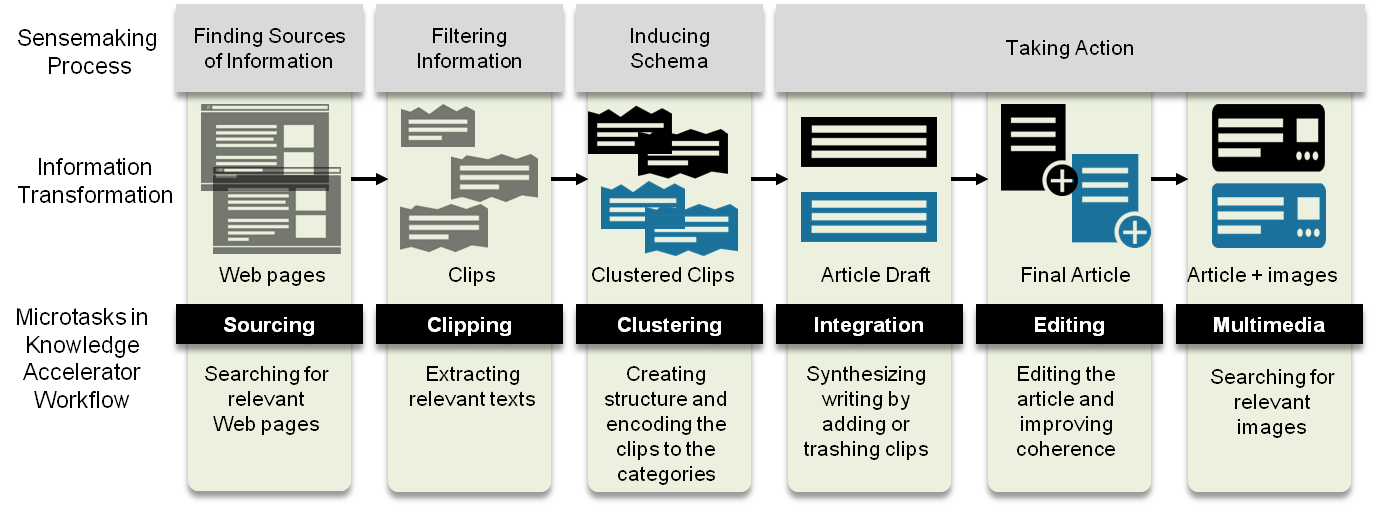
\includegraphics[width=1\columnwidth]{Chapters/KA/overview}
    \caption{The process of the Knowledge Accelerator (KA), from start to finish}
    \label{fig:process}
\end{figure*}

\section{System Architecture}

%The ``Knowledge Accelerator'' (KA) is a prototype system which uses crowd workers each contributing small amounts of effort to synthesize online information for complex and/or open-ended questions. The Knowledge Accelerator system starts with a given question (such as ``How do I deal with the arthritis in my knee as a 28 year old'') and crowdsources the generation of a coherent article that synthesizes different sources, viewpoints, and topics found online relevant to answering the question.

%Critically, the KA system accomplishes this process without a core overseer or moderator. \niki{I think this is the part we should remove / consolodate with intro} The aim of the system was to probe how to accomplish a complex information synthesis task entirely through relatively small contributions. We operationalized this intention by limiting our maximum task payment to \$1 US, aimed at incentivizing a target task time of approximately 5-10 minutes. We chose this approach because a fixed payment amount matches the structure of many microtask crowdsourcing markets (e.g., versus a fixed time period of 10 minutes). While some crowdsourcing markets (such as UpWork or eLance) do support hourly rates and fixed time periods, the double-sided transaction (or ``handshake'') costs in which employers and workers vet each other in such markets would constitute a substantial fraction of the working time we target, and the time scale of projects in such markets (typically measured in hours) do not match well with the time scale of the projects we target here (i.e., minutes).

%An example of the output of the system for the target question ``How do I get my tomato plants to produce more tomatoes?'' can be found in Figure~\ref{fig:final_answer}. To produce this output workers find high value sources from the web (e.g., gardening.about.com), extract the useful and relevant clips of information from them, cluster these clips across sources into commonly discussed topics (e.g., feeding or pruning), and generate an article for each topic that synthesizes the relevant clips into coherent chunks of information while reducing redundancies (e.g., if several sources all mention soil pH range, the article should not include that information multiple times). Workers also find relevant multimedia images and video to illustrate each chunk. Information sources used in the creation of the article are referenced in the final output, and the article is organized by subtopics with the most diverse set of references first (See Figure \ref{fig:process} for the KA process overview). 

%The above tasks of finding, filtering, organizing and generation can be though of as two larger steps: learning a good structure for the article based on sampling information from different online sources, and developing a coherent digest given that structure. To learn a structure workers find high quality online sources and clip relevant pieces of information, which are clustered into topics or categories. The information for each topic is then synthesized into a coherent digest through two steps: first integrating information within a topic, and then enforcing consistency across topics. Below we discuss the challenges involved in developing the system,  particularly focusing on issues central to supporting big picture thinking with workers each seeing only a small part of the whole. We then evaluate the utility of the system’s output versus top online sources across a variety of topics.

%\michelle{at this point, I feel like I'm missing a general overview of what exactly happens... then we have the challenges that all kind of fit together but I don't have a good structure put them into. I guess the figure kind of does this, but possibly a list in the text with a little more description would help me out} \niki{good point. nathan can you add back in a concise 2-3 sentences getting across the essence of the process, maybe noting that we are taking the stages from sensemaking but doing them in a breadth-oriented instead of an iterative way?  i'd suggest putting that description right before this paragraph}\niki{actually cancel that, i'll work on restructuring this whole part to address this better}

Broadly, there are two hard problems involved in crowdsourcing information synthesis: learning a good structure for the article based on sampling information from different online sources, and developing a coherent digest given that structure. Below we discuss how the system addresses each of these problems in turn.

%To learn a structure workers find high quality online sources and clip relevant pieces of information, which are clustered into topics or categories. The information for each topic is then synthesized into a coherent digest by integrating information within a topic, and then enforcing consistency across topics.


\subsection{Inducing Structure}

How can a crowd learn a good structure for an article on an arbitrary topic? Previous crowd approaches such as CrowdForge or CrowdWeaver \cite{kittur2011crowdforge, Kittur:2012:CVM:2145204.2145357} required workers to decide on a structure up before collecting information on each of these topics. However, these approaches fail when the structure must be learned from the data. For example, few workers will know what the subtopics should be for fixing a Playstation’s blinking light or for dealing with arthritis; instead, the appropriate structure should emerge from the data. A single individual making sense of a topic often engages in an iterative process of sampling data and building a structure; however, to reduce the latency of having multiple cycles we explore an alternate approach in which the crowd samples a large amount of data in parallel, then leverage a novel hybrid crowd-machine approach that clusters information into topics without requiring any one worker to see the whole picture.

%induce a structure from that.  a lot of data, use  we first employ crowd workers to find and filter relevant online information. However, as this can collect more information than a single worker could process, we introduce a hybrid

%Research on how people make sense of information online for themselves as they learn new subjects suggests that people go through an iterative sensemaking process in which they are continually finding information about a subject and inducing or refining a structure from the information they found [cites]. Previous approaches such as CrowdForge and CrowdWeaver \cite{Kittur:2012:CVM:2145204.2145357, kittur2011crowdforge} have done a variation of this by having workers decide on an information structure up front, such as what topics should go into an article about New York City (e.g., attractions, economy, etc.), and then other workers search for information on each of these topics. 

%However, it appears that if structure is induced too soon from too few pieces of information, the resulting structure tends to be more poorly formed than if a rich set of information is first collected. Additional research suggests that instead of deciding on a set of topics first and then seeking information for them, one should first seek information and then decide on the set of topics based on what that information contains. Basing the structure on a larger set of online sources has multiple potential advantages: increased coverage of topics, reduced impact from lack of worker prior knowledge (as the knowledge is coming from the sources), and knowledge of which topics are common across many sources (perhaps indicating importance or widely shared viewpoints). For example, in the Playstation scenario described above workers may encounter many possible solutions they wouldn’t have prior knoweldge of, and be able to see which solutions seem to be more commonly cited which might suggest trying them first over solutions that are only mentioned by a single source.

%While there may be multiple benefits, the challenge of crowdsourcing the "seek first - structure later" approach is that much more information is collected for the structuring phase than an individual might easily process at once. Splitting this information up so that each worker only sees a small piece can lead to problems with coming up with good structure; for example, a worker in the above Playstation example might see a solution talking about overheating and, without context of the other solutions, categorize it under overheating. However, if they were to have a global overview of the information, they would know that all the solutions talk about overheating, because that is what the actual problem, and a better category would be the solution type. 

%In a crowdsourced version, workers may not know what the topics should be and the structure of the resulting structure will be missing important topics or focusing on less important topics. For example, in writing an article about approaches to fix a Playstation 3’s blinking yellow light, while there is much information available online about the subject most workers will have little prior knowledge on which to base their judgments of what to include in the article and how it should be structured.

%We describe an approach to addressing this problem below, in which crowd workers first search for and filter information to generate a rich set of data, then a hybrid crowd-machine approach enables clustering the information into topics without having any one worker seeing the whole picture.

\subsubsection{Finding Sources}
To search for and filter high quality information sources we asked five workers to each provide the top five web pages relevant to the target question. We found these numbers to work well in practice; future work using optimization approaches \cite{Kamar:2013:LET:2484920.2485011} could potentially set these dynamically. To ensure high quality responses, for each source we asked workers to report the search term they used and provide a small text clip as ``evidence'' showing why the source is helpful. This approach appeared to be successful in encouraging workers to find high quality sources: workers made on average 2 different queries ($\sigma = 0.3$), and their more commonly cited sources covered more categories of the structure with fewer sources than choosing sources using standard information retrieval approaches (i.e., using the MMR diversity-based re-ranking algorithm to reorder the sources gathered from the crowdworkers \cite{carbonell1998use}). Sources cited by at least two workers were sent to the filtering stage.


%This requires them to browse through each of the sources to gain more understanding of the context, and also encourages them to reformulate their searches to find better sources. 

%Initially, we considered using just the top search results for a particular question as the input for the structure induction stage. However, because we wanted to collect a diverse set of sources, we thought that crowd workers given the ability to perform their own queries might discover a better article set. We conducted a preliminary study where we used the MMR diversity-based re-ranking algorithm to reorder the sources gathered from the crowdworkers \cite{carbonell1998use}, to see if we could cover as many categories extracted in the structuring phase with fewer sources. However, results showed that the original order ranked by crowdworker citation count still covers more categories with fewer sources, indicating that crowdworkers are using good queries and providing valuable judgements when picking sources from the their search results.

%From our experiments, crowdworkers use an average of 1.98 queries ($\sigma = 0.288$) to find the five sources, and find sources that provide more categories with fewer sources than standard information retrieval approaches.

\subsubsection{Filtering Information}

%Each source could contain a variable amount of information relevant to the target question. Some long pages may have very many chunks of relevant information that would exceed the capacity of a single of our tasks, while other pages of the same length may have only a few.  
To filter relevant information snippets from each source workers were presented with one web page and asked to highlight and save at least five pieces of information that would be helpful for answering the question using an interface similar to that described in \cite{kittur2013costs} (Figure~\ref{fig:clipping}). One challenge we encountered was that each page could contain a variable amount of useful information, with some long pages having more snippets than a single worker would extract. To spread out worker coverage on long pages, we showed workers sections that had been highlighted by previous workers and asked them to first look for unhighlighted areas when choosing clips. This preference for novelty and surfacing prior workers' effort allowed us to engage multiple workers for tasks with an unknown amount of relevant information in a more efficient way than simply letting loose many independent workers who would overly focus on the beginning of the page, or having some workers start at the beginning and others at the end \cite{bernstein2010soylent}. To focus more effort on potentially rich sources the system dispatches two workers to each source with an additional two workers for every two additional citations a source received.

\begin{figure}[!ht]
    \centering
    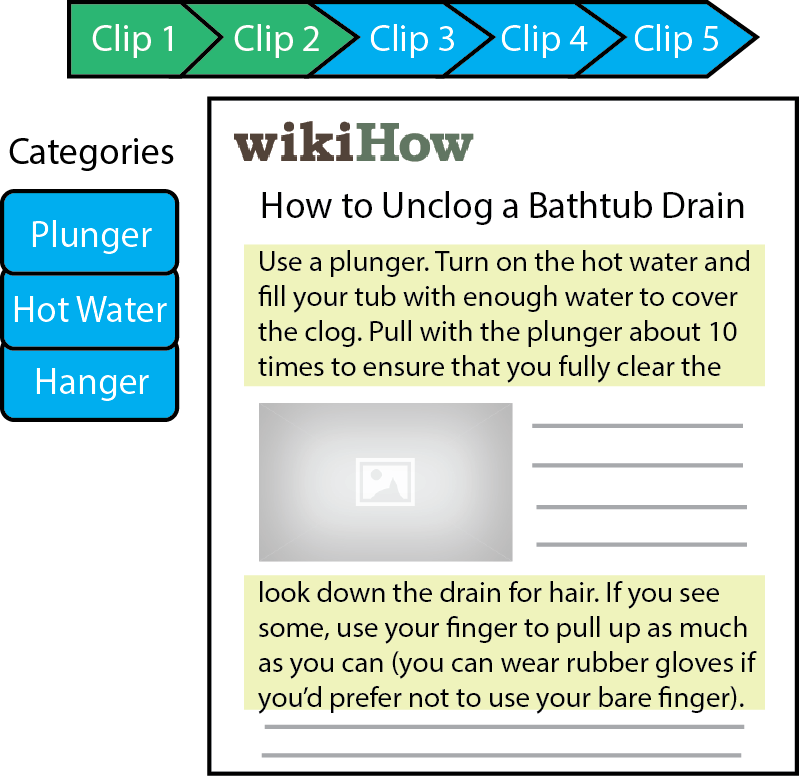
\includegraphics[width=0.5\columnwidth]{Chapters/KA/clipping}
    \caption[Crowdworkers extract and label information from webpages]{Workers extract 5 different pieces of relevant information from pages and give it a label}
    \label{fig:clipping}
\end{figure}

%Sources cited by at least two workers were sent to the clipping phase, where workers extracted from them useful and relevant clips . 

%The idea behind this is that multiple sources will contain overlapping solutions, and in later stages we want to synthesize information for the same solution across different sources. 

%One challenge was maintaining the distribution of information, making sure popular sources are sure to have enough information extracted from them, while still ensuring that a large variety of information is captured. Previous solutions, like "find-fix-verify" \cite{bernstein2010soylent} use a large number of crowd workers and variance for coverage. Instead, to address this, two clipping workers were dispatched initially to any source that reached this citation threshold, with an additional two workers dispatched for every two extra citations a source received. Each worker was presented with one web page and asked to highlight and save at least five pieces of information that would be helpful for answering the question using an interface similar to that described in \cite{kittur2013costs}. To spread out worker coverage on long pages, we showed workers sections that had been highlighted by previous workers and asked them to first look for unhighlighted areas when choosing clips.

Initially we had workers provide labels to categorize each clip, which we planned to use to develop a structure for the article. However, the lack of context of the bigger picture made these labels poorly suited for inducing a good structure. For example, in Figure~\ref{fig:delayed-structuring} the top box shows the category structure induced from labels generated during clipping, while the middle and bottom boxes show the structure induced from the subsequent clustering phase and from a gold standard developed by two independent annotators with access to all clips and sources, respectively. Categories induced from the clipping labels poorly match the gold standard, and include categories with very different abstraction levels (e.g., \textit{Use Drano Max Gel} vs \textit{tips}). This motivated the development of the subsequent clustering phase.

%During this saving process, the worker was prompted to supply a category label for each piece of information they saved. These labels were used only as a work check to control the quality of the clips due to the limited context that each worker had while creating them. Initially, we had planned to use these labels as a way to categorize information for later stages. However, the lack of context of what future clips would be made caused early clip workers form providing labels that ended up serving as poor organization structures. This then caused low quality categories to propagate as new workers used them. This problem aligns with previous research on taxonomy cascades \cite{kittur2014standing,kittur2013costs}, suggesting that we should delay structuring in order to effectively find the proper categories, which motivated the development of the structuring phase described next.

 \begin{figure}[!ht]
 	\fbox{ \vbox{
 		\ttfamily
 		\footnotesize
 		
		\textbf{categories induced during clipping:}\\
 		Boil Water, use hot water, Plunger, try a snake, How to Remove drain stopper, bleach, Use Drano Max Gel, baking soda, drain, tips to unclog, problem, tools, research, internet research, ..., etc.
 		
 		\rule{\columnwidth}{0.1pt}
 		
 		\textbf{categories induced after clipping:}\\
 		Hot Water, Plunge, Plunger, Snake the Drain, Remove the Drain Cover, Drain Cleaner, Remove Hair Clusters.
 		
 		\rule{\columnwidth}{0.1pt}
 		
 		\textbf{annotator categories:}\\
 		Hot Water, Plunger, Plumbing Snake, Remove Cover, Chemicals, Bent Wire Hanger, Call a Plumber, Shop Vacuum.
 	}}
 	\caption[Categories induced from different stages of KA.]{Categories induced from different stages for Q1: \textit{How do I unclog my bathtub drain?}}
 	\label{fig:delayed-structuring}
 \end{figure}

%To demonstrate the difference in category quality during vs. after clipping, in Figure~\ref{fig:delayed-structuring}, we show 1) categories generated by crowdworkers during clipping, where each crowdworker can create new categories or reuse categories created by other workers, 2) categories created after the clipping phase and with the structure induction phase, and 3) categories created by two independent annotators who had access to all the clips and their original sources. The categories generated during clipping are of very different abstraction levels (e.g., \textit{Use Drano Max Gel} vs \textit{tips}), while categories generated after the clipping phase are more coherent and more consistent with the expert categories.

%\begin{figure}[!h]
%    \centering
%    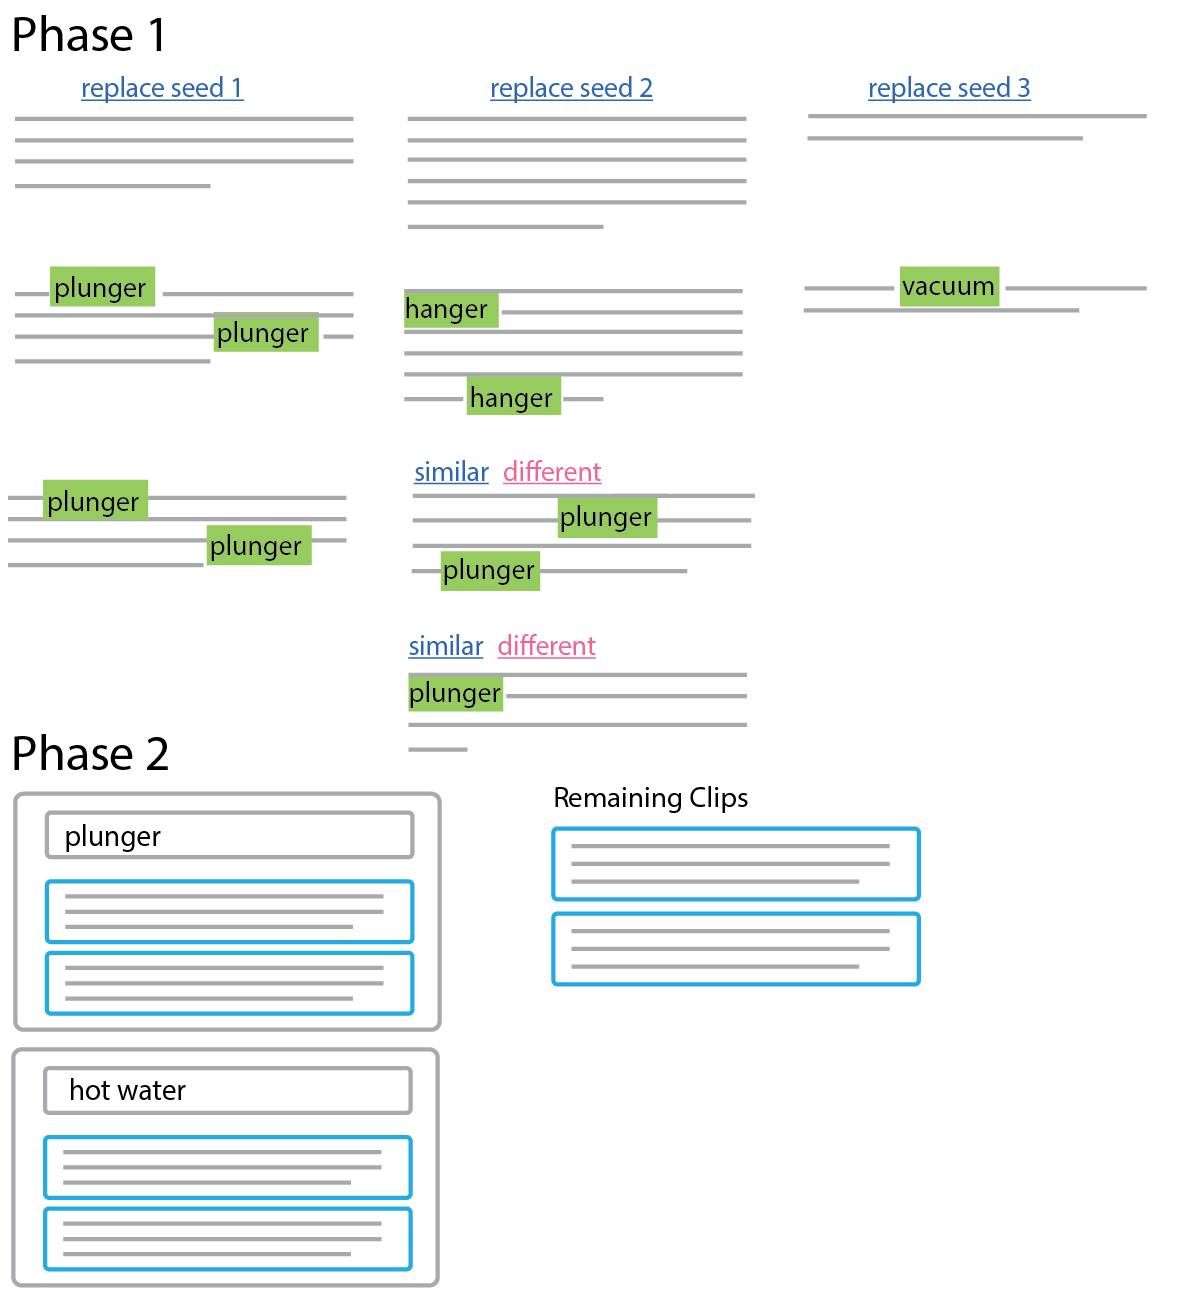
\includegraphics[width=0.9\columnwidth]{clustering-02}
%    \caption{In phase 1 workers identify different seeds and keywords to used in automatic clustering. In phase 2, workers clean up the clusters and name them.}
%    \label{fig:clustering}
%\end{figure}
\subsubsection{Clustering}

%The structuring phase takes all of the clips produced from the clipping phase and tries to extract a categorical structure from them. The motivation behind this is so we can 1) synthesize overlapping information across sources, 2) present the user with different solutions as article sections, and 3) generate smaller sets of clips of the same category so that they are more manageable in the later synthesis stages. The challenge here differs from most crowd-based systems where the tasks can be naturally broken down into smaller pieces, such as labeling images with predefined classes. 

Inducing categories in unstructured collections of text typically requires understanding the global context in order to identify categories that are representative of the information distribution and at appropriate levels of abstraction. The problem of inducing structure without any single worker having a full global context is a particularly challenging problem, and although we describe a basic solution to the problem here for reasons of space and scope, we present a more sophisticated distributed approach in \cite{alloy} that further generalizes the problem to other domains.

%(Figure~\ref{fig:clustering}). 
Our approach takes advantage of the fact that many real world datasets have long-tailed distributions, where a few categories make up the bulk of the head of the distribution and many categories with few instances make up the tail. The intuition behind our approach is that first, the crowd can act as a guide to identify the large categories in the head of the distribution, with their judgments training a classifier to categorize the easy cases with high confidence. After automated classification, the crowd can again be used for ``clean up'', covering the low-confidence edge cases in the tail of the distribution. This also has the added benefit of easily breaking up the larger question context into sub-contexts for easier consumption in the later parts of the system. 

In the first phase, we use workers to label a number of representative categories and leverage those labels to identify meaningful features for an automated classifier. One critical challenge is that workers need to obtain a sense of the distribution of the data without seeing it all. To accomplish this we developed a design we call open-ended set sampling in which workers are presented with four random clips as seeds, and are asked to replace them repeatedly with another random clip until they can determine that the four seed clips belong to meaningfully different categories. Therefore, not only do they have to read the information present in the initial seed clips, but they also need to sample multiple times to understand what ``different topics'' mean for this dataset. In doing so they are randomly shown new clips, which means they are more likely to encounter categories with probability matching the distribution of topics in the data (i.e., higher probability of encountering larger categories).

After workers pick the seeds, we ask them to highlight discriminative keywords in each of the seed clips which are used to query for similar clips from the full dataset, which the workers then label as as \textit{similar} or \textit{different}. With the keyword highlights and the labels created by the workers, we use an SVM classifier and hierarchical clustering to cluster the high confidence portion of the dataset, sending the uncertain instances to Phase 2. 

%One important pattern embedded in the above design is that we leverage worker choice in order to find the clips and keywords that can strongly distinguish between clusters. We accomplish this by indicating to workers that they will have to find similar clips to their initial seed clips, which encorages them to pick good keywords because it helps them reduce their own future workload.

In the second phase, we employ crowdworkers to clean up the output of the classifier, by presenting them the existing clusters on the left of the screen, and the remaining clips on the right. The workers are first familiarized with the clusters by asking them to review the clips in each cluster and give it a short description. They then categorize the remaining clips into existing clusters or create new clusters if no existing cluster is relevant. These categorization judgments are used to refine the hierarchical clustering model.

%This process of evaluating then acting ensures the workers have some understanding of the current context first, so that they can assign clips to the most suitable category, and also to create coherent categories if they need to.

\subsection{Developing a Coherent Article}

%After having induced a structure for the question, there are several possibilities for using the information. For some purposes (e.g.,  \cite{Chilton:2013:CCT:2470654.2466265, kittur2014standing}), it would be enough to just report the categories and associated clips. However, there are benefits to having an article, such as easier consumption, a coherent flow of information, and the inherent organization of information that might not be present in a cluster of short clips.

%The previous section described how to take an online topic area and develop a big picture of its structure through only local views. The output of this process is a set of topics and a set of clips for each topic. 

In this section we describe a set of processes which take as input a set of topics and clips for each topic and output a coherent Wikipedia-like article. There are two core challenges in doing this: first, creating coherence within a topic (e.g., consolidating redundant information); and second, creating coherence between topics (e.g., maintaining consistency across sections). 
%First, we achieve within topic coherence by having individuals integrate the pieces of information within a topic. Second, we have individuals edit the flow of each topic to improve its consistency and coherence with the other sections. 

\subsubsection{Integration}

Within a single topic, there may be many clips which all contain substantively identical information (e.g., the ideal pH level of soil for growing tomatoes); one goal is to reduce this redundancy so that the final article only describes this information once. At the same time, we recognize the value to seeing that multiple sources all say the same thing; thus, we would like to keep track of all the sources that mention a particular chunk of information. Furthermore, tracking source provenance allows the user to drill back to the original information source in case it is described inaccurately or in a biased way.

To accomplish this we developed an interface in which workers were presented with 5 random clips of information for a given subtopic and asked to integrate that information into a shared text pad. Specifically, they were asked to write the gist of the clip in their own words and transfer the provenance of the clip as a footnote. Missing footnotes triggered a verification check.

Initially, we just instructed individuals to cluster similar items together and insert only the footnote for redundant information. However, we noticed that workers were reluctant to change what they perceived as another worker’s contributions, consistent with the social blocking found in Andre et al. \cite{andre2014effects}. This developed into a larger challenge: How could we get workers to gain an understanding of what was in the existing shared pad and feel comfortable modifying it? We introduced a technique we call evaluate then act that requires individuals to read what others have already put into the integrated answer before they are allowed to make a decision about the clip. Our final interface prompts workers to provide specific line numbers corresponding to existing information relevant to their clip, or to explicitly mark their clip as new information or trash. Compared to a version of the system without this structure, significantly more clips were inserted into the middle of the pad to align better to their given section (13\% more, $t(24) = 2.568$, $p < 0.05$) or excluded (11\% more, $t(24) = 4.592$, $p < 0.01$) when workers were asked to evaluate before acting.

%The biggest challenge faced in doing so was encouraging workers to engage in the cognitively demanding task of mapping their clip's information to the information already in the pad, which might include functionally the same information content but in different forms. 
%One challenge with removing redundant information is a relatively subtle but ubiquitous social factor in crowd work: that workers are wary of interacting with other workers’ contributions. [territoriality in wikipedia, difficulty in getting workers to interact and edit each others’ work in andre-limerick writing]. 

\begin{figure}[!ht]
    \centering
    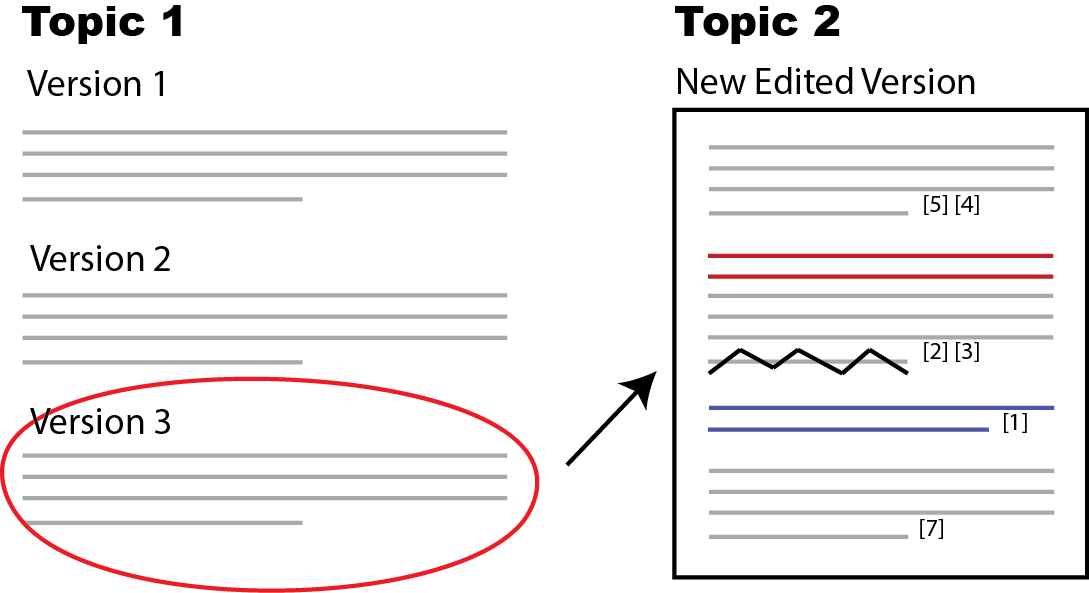
\includegraphics[width=0.6\columnwidth]{Chapters/KA/edit}
    \caption[The 'vote-then-edit' pattern promotes consistency and motivates workers.]{Editing uses the 'vote-then-edit' pattern to promote consistency and motivate workers}
    \label{fig:editing}
\end{figure}

\subsubsection{Editing}

We also noticed that coherence needed to be managed not only within topics, but between topics as well. A number of between topic inconsistencies became apparent during the development process, ranging from formatting to structuring to prose. For example, some topics would be organized with bullet points versus paragraphs, and some in the second person point of view versus third person. Previous crowdsourcing approaches have trouble dealing with cross-topic consistency because reading even a single topic can take significant time, let alone reading and editing across all topics. For example, CrowdForge's \cite{kittur2011crowdforge} approach simply concatenates topics into an article without any attempt at maintaining global coherence. This approach can succeed if the topics and structure either do not require consistency or if they are extremely well specified beforehand: in CrowdForge and CrowdWeaver defining a science article “template” with clear sections such as \textit{what is the problem, what the researchers did}, accomplishes this effectively in a similar manner to core editors specifying a structure in Wikipedia that peripheral members then fill in \cite{kittur2008harnessing}. However, in the general case such well-defined and pre-specified templates are not always available.

%The decision to \textbf{delay structuring} of the Integration task created the need for a task to make the output cohesive and error-free.  Instead, workers would often place their contributions next to existing contributions leading to redundancy (despite instructions to remove redundant text). On average, about 36\% ($\sigma = 0.261$) (using word Levenshtein distance) of the initial pad was modified during editing, suggesting that substantial portions of the pad still merited revision. Another challenge was making each subtopic consistent with other subtopics, as the Integration phase kept each subtopic independent.

To address this we introduced a new pattern which we call vote-then-edit (Figure~\ref{fig:editing}). This pattern asks workers to first review and vote on and choose the ``best'' version of a subtopic created by previous workers, while simultaneously getting a sense for commonalities in style, grammatical choices, and organization. They proceed to edit a new subtopic (phase one) or improve on the item they voted on (phase two). In the second case, we expected workers would more carefully select the best version to reduce their future workload, as well as be more motivated to fix issues in it because they had a choice in what they wanted to do. 

We used the vote-then-edit pattern in an interleaved ``horizontal'' and ``vertical'' workflow. The horizontal phase uses the refined and edited versions of a subtopic section as a ``model'' for improving the rough output from the integration phase for another subtopic section. Specifically, three workers vote on which of three versions of an edited subtopic section is the best and then edit a different subtopic subsection using their answer from voting as a model. Their resulting edited output is sent to the vertical phase, in which three workers vote on which of those versions is the best, and are then asked to further improve this now with all of the other subtopic paragraphs presented to them, to ensure the current subtopic has good flow with the other sections. The output from these workers is used in a new horizontal phase, and the cycle continues.  The intuition here is that the horizontal phase provides only a single section as a model since there is substantive editing work remaining that requires relatively limited context, while the vertical phase provides all sections because the primary editing work remaining is ensuring consistency across sections. Splitting editing into two interleaved phases with different context-work tradeoffs appeared to be more effective than an older editing approach with a single phase. When we compared the evaluation ratings for the older editing to the interleaved vote-then-edit approach for two questions (Q1 and Q2 in Table \ref{tab:evaluation} respectively), the newer answers were found to be significantly more understandable ($\bar{x} = 0.457$, $p < 0.01$) and helpful ($\bar{x} = 0.373$, $p < 0.05$), suggesting this design pattern helped to create more coherent output.


%Therefore, we had two challenges: ensuring a consistent format between sections, and creating a global article flow from topic to topic. Editing was divided up into two phases to tackle these problems separately: an initial editing phase where a worker revises the output from the integration task, and a subsequent consistency phase where individuals are tasked with making the output coherent with other subtopics. In the first phase, a worker votes on the output of a different subtopic's editing phases to choose the ``best'' version. They then are presented with a different subtopic section and asked to improve it, using their answer from voting as a model. In the second phase, individuals vote on the output from the first phase, and are then asked to further improve this now with all of the other subtopic paragraphs presented to them, to ensure the current subtopic has good flow with the other sections. The output from these workers is then used in a different subtopic's first phase, and the cycle continues. This workflow, which we call vote-then-edit (Figure~\ref{fig:editing}), forces workers to read through another topic, and have a sense for its style, grammatical choices, and organization. Additionally, we expected individuals would more carefully select the best version to reduce their future workload, as well as be more motivated to fix issues in it because they had a choice in what they wanted to do. We compared the evaluation ratings for the older editing to the newer editing using this approach for two questions, the bathtub question and the tomato question (Q1 and Q2 in Table \ref{tab:evaluation} respectively) . The newer answers were found to be significantly more understandable ($\bar{x} = 0.457$, $p < 0.01$) and helpful ($\bar{x} = 0.373$, $p < 0.05$), suggesting this design pattern helped to create more coherent output.

\subsubsection{Multimedia}

Images and video can help the reader skim and digest information quickly, as well as provide rich information such as diagrams, instructions, and how-to examples. In our system we enable multimedia from diverse sources to be tied to information blocks, which we define as sections of text demarcated by footnotes. Informally, information blocks correspond to units of information, such as steps in a how-to, or statements or evidence. This has the benefit of ensuring that the images found are specific to pieces of information found in the answer, rather than just being general to the subtopic. For the version of KA described here we did not employ redundancy or voting in the multimedia stage as we did not encounter quality issues; however, since multimedia enrichment is not a particularly interdependent task existing known quality control approaches such as redundancy and voting \cite{kittur2013future} would likely be sufficient for a production system.

\section{Design Patterns}

As mentioned in the above task descriptions, during our iterations on each stage we ended up introducing several design patterns that improved the output. Each phase had its own distinctive challenges, yet they still suffered from some of the core challenges highlighted by previous work: motivation, quality-control, and context \cite{kittur2013future}. Our design patterns served to guide our final system design and add to the set of crowd patterns introduced by previous research \cite{kittur2011crowdforge,bernstein2010soylent,kittur2013future,little2010turkit,bigham2010vizwiz,lasecki2012real,kulkarni2011turkomatic}. They may be particularly relevant for challenges involving complex interdependent tasks requiring global context for workers seeing only local views. 

\subsection{Context before Action}

One of the biggest challenges in crowdsourcing a complex, interdependent task such as information synthesis is providing workers with sufficient global context to perform well despite them having only a local view. Previous researchers have suggested a variety of useful patterns related to this goal, including making the cost of spurious answers as high as valid ones \cite{kittur2008crowdsourcing}, identifying and surfacing specific sub-task dependencies \cite{kulkarni2012collaboratively,retelny2014expert}, unified worker interfaces \cite{zhang2012human} and re-representing tasks in simplified forms \cite{andre2014crowd,Kittur:2012:CVM:2145204.2145357}. We contribute a set of patterns adding to this literature, specifically focusing on a key tradeoff: given a limited amount of time and effort for an individual worker, how can we provide workers with global context (i.e., investing in their ability to make better decisions) but also engage them in actual production work? Too much invested time providing context reduces the amount of time available for improved task performance.

%One of the primary decisions we had to make was how much context we should provide to workers at each step , and how to convey that context to workers in a meaningful way. 

%In the topic identification and clustering phase, there are three different implementations of this pattern. 

\textit{Open-ended Set Sampling.} One challenge with large datasets is giving workers a sense of the distribution of the data despite their observing only subsets of it. This pattern involves a comparison task in which workers are asked to sample random items from the data in order to create a set of non-matching items, as seen in the first step of clustering. A key design factor in this pattern is having a good set function that provides a driver for open-ended sampling and also a stopping point (e.g., when a worker's familiarity with the distribution gives them a sense that their four seeds represent substantively different topics in the dataset).

%\textit{Signal By Doing} In order to get workers to understand the context provided to them, we designed evaluation mechanisms at the beginning of their main task that would both allow them to gain a procedural understanding of their task as well as process the context information produced by other workers. This was a particularly useful pattern, seen in the clustering, integration, and editing phase. In integration, workers had to process previous information in a very specific way so they would both do a specific procedure as well as understand what other workers had done. In editing and clustering, workers had to do a smaller, context-priming task (voting and labeling, respectively). 

\textit{Evaluate then Act.} In order to get workers to understand
the context provided to them, we designed evaluation mechanisms
at the beginning of their main task that would allow
them to get acquainted with the output from previous workers.
This helped workers understand how previous workers
processed the information provided to them, improving consistency
of the output on parallel tasks, and reducing repeated
information. This pattern was leveraged in a number of tasks: clustering, integration, and editing. In the integration phase, we
additionally used the evaluation phase to signal to workers that removing others' work was acceptable and expected, showing that it could be useful in socializing workers into desired procedural practices as well as providing them with context.

\subsection{Tasks of Least Resistance: Leveraging Worker Choice}

Since workers were mostly dealing with dense textual information on a topic they were likely unfamiliar with, we wanted to ensure they were sufficiently motivated. Therefore, we developed a pattern that doubled as both a quality control measure, we well as an incentive for workers. The ``task of least resistance'' pattern requires that the same crowd worker be involved in two stages of the task, a first stage in which they choose what to work on from a number of alternatives (e.g voting) and a second stage in which they themselves benefit from their choice in terms of having to do less work, easier work, or being able to submit a higher quality output. The intuition is that to minimize their later work workers will choose a foundation that requires the least amount of work possible; i.e., they will choose the ``task of least resistance''. This act of choosing is intended to also provide workers with a sense of agency and purpose, which has been shown to increase task performance \cite{chandler2013breaking, rogstadius2011assessment}. This choice also has the potential to increase task performance through workers trying to avoid cognitive dissonance: since workers have themselves presumably chosen the best quality work to start, poor quality final output could reflect on their own worth \cite{weick1964reduction}. This has a trade off of potentially making tasks longer, more complicated, and more expensive, however the benefit is a higher quality output. 

%\subsection{Capturing a Distribution}

%An important part of information synthesis is gathering enough diverse information, while still noting what information is commonly considered to be "better". This is akin to a capturing a distribution: you need to understand which information is more popular, however you need to make sure to still gather the tail information as well. This is not just an issue with information synthesis, understanding distributions is a problem in other domains such as [X, Y, Z]. With enough sampling with crowds, eventually you obtain the desired distribution. However, in order to accomplish this more efficiently, we assign workers for a preference for information novelty and only once the most novel information has been noted, do they recapture the more popular information. This, coupled with assigning more individuals to more "popular" informational sources, creates a biased sampling process that captures all of the information, and then selects a limited portion of the head of the distribution to really promote. 

\section{Implementation}

The main portion of the application was built using Ruby on Rails and integrated with Amazon's Mechanical Turk through the Turkee ruby gem \cite{turkee}. The Ruby on Rails application served as the primary user interface for both the question asker, crowd worker, as well as the answer viewer. A question posed to the system would start the workflow, beginning with source finding. For each stage, after a certain set of conditions were met (number of sources, clips, completed clustering, etc.), the next task in the workflow was automatically started. This allowed the system to run through the entire process with minimal intervention. 

The clipping task utilized Readability's parser API to simplify the appearance of the sources provided during the sourcing phase. This allowed workers to view a cleaner interface in which to clip from, and it also removed some technical limitations involved with clipping from pages that might be multi-paged (readability combines these into one long document) or featured heavy javascript functionality that would interfere with the clipper tool. 

For the first phase of the structure induction tasks, the TfIdfSimilarity ruby gem is used for searching clips similar to the seed clips \cite{rubytfidf}. LIBSVM is used for combining the crowd judgments and cluster a large portion of the dataset \cite{chang2011libsvm}. For the integration and editing tasks, we utilized the Etherpad-lite text pad library \cite{Etherpad} to allow workers to simultaneously work on the same output.

\section{Evaluation}

To evaluate the usefulness and coherence of the system's output we compared it to sources an individual might use if they were to complete this task without the KA system. This would most likely involve the use a search engine such as Google to gather information and use existing information sources to learn about the topic. Therefore, as an evaluation, we had a separate set of crowd workers perform a pairwise comparison of the KA output to that of top results returned by Google and those found useful by multiple crowd workers.

\subsection{Method}

Participants were recruited through the AMT US-only pool and paid \$1.50 for the evaluation task. Each participant was randomly assigned to compare the output from the KA system with an existing top website for that question. An individual could only provide one rating per question, but could do the rating task for more than one question. We removed 34 of the 1385 unique participants who provided an evaluation rating who also participated in a KA system task.

The ``top websites'' used in the comparison task were the top five Google results, as well as any additional Google results that were highly cited (mentioned by 3 or more turkers) during the sourcing phase of the system. Some questions had a larger number of highly cited sources, resulting in more additional websites, as can be seen in Figure~\ref{fig:aggregated}.

In the evaluation task, participants were first asked a series of questions that would cause them to read and understand both sources. In order to encourage quality through defensive task design \cite{kittur2008crowdsourcing}, for the output from the KA system and the existing web page, they were asked to list the different sections on each and three different keywords that would describe those sections. After they read and parsed each web page, they were presented with a brief persona of a friend who was having the problem posed to the KA system. Workers were then asked, for that problem, to rate the comprehensiveness, confidence, helpfulness, trustworthiness, understandability, and writing of each web page on a seven point Likert scale (from 1 to 7) and provide an explanation for their rating on each dimension. We averaged ratings on these dimensions into a single score representing the overall perceived quality of the page.

We selected 11 target questions for evaluation by browsing question and answer forums, Reddit.com, and referencing online browsing habits \cite{pewReport}. For some questions, we added some additional constraints to test the performance of the system for more personalized questions. In addition to this external evaluation, we also had the crowdworkers who participated in the KA system fill out a short feedback form detailing their experience using the system. We ask three questions about the difficulty of the task, the clarity of the instructions provided, and the easy of use of the user interface. We recorded some brief demographics about our workers, including to the country they were from.

\begin{table}
  \centering
  \footnotesize
% question, number of sources, number of clips, number of turkers
  \begin{tabular}{l r l}

	Question &
	\multicolumn{1}{c}{N} &
    \multicolumn{1}{c}{Score} \\
    \hline
	% 102
	\multicolumn{1}{p{0.75\columnwidth}}{\textbf{Q1}: \textit{How do I unclog my bathtub drain?}}
	& 116 & ~0.292 * \\

	% 115	
	\multicolumn{1}{p{0.75\columnwidth}}{\textbf{Q2}: \textit{How do I get my tomato plants to produce more tomatoes?}}
	& 177 & ~0.420 * \\

	% 153
	\multicolumn{1}{p{0.75\columnwidth}}{\textbf{Q3}: \textit{What are the best attractions in LA if I have two little kids?}}
	& 158 & -0.044 \\

	% 116
	\multicolumn{1}{p{0.75\columnwidth}}{\textbf{Q4}: \textit{What are the best day trips possible from Barcelona, Spain?}}
	& 98 & -0.109 \\

	% 177
	\multicolumn{1}{p{0.75\columnwidth}}{\textbf{Q5}: \textit{My Worcester CDi Boiler pressure is low. How can I fix it?}}
	& 139 & ~0.878 * \\

	% 168
	\multicolumn{1}{p{0.75\columnwidth}}{\textbf{Q6}: \textit{2003 Dodge Durango has an OBD-II error code of P440. How do I fix it?}}
	& 138 & ~0.662 * \\

	% 175
	\multicolumn{1}{p{0.75\columnwidth}}{\textbf{Q7}: \textit{2005 Chevy Silverado has an OBD-II error code of C0327. How do I fix it?}}
	& 135 & ~0.412 * \\

    % 160
	\multicolumn{1}{p{0.75\columnwidth}}{\textbf{Q8}: \textit{How do I deal with the arthritis in my knee as a 28 year old?}}
	& 139 & ~0.391 * \\

    % 161
	\multicolumn{1}{p{0.75\columnwidth}}{\textbf{Q9}: \textit{My Playstation 3 has a solid yellow light, how do I fix it?}}
	& 119 & ~0.380 * \\

    % 162
	\multicolumn{1}{p{0.75\columnwidth}}{\textbf{Q10}: \textit{What are the key arguments for and against Global Warming?}}
	& 138 & ~0.386 * \\

    % 163
	\multicolumn{1}{p{0.75\columnwidth}}{\textbf{Q11}: \textit{How do I use the VIM text editor?}}
	& 138 & ~0.180 \\
    \hline
    \multicolumn{3}{l}{\textbf{*} = significant at $p < 0.01$ after Bonferroni correction}\\

  \end{tabular}
  \caption[Comparing KA output with top websites for the eleven questions.]{Average difference between the KA output and top websites for the eleven questions (positive indicates higher ratings for KA, negative indicates higher ratings for the competing website). Each rating was an aggregate of 6 questions on a 7-point Likert scale.}
  \label{tab:evaluation}
\end{table}

\begin{figure*}
    \centering
    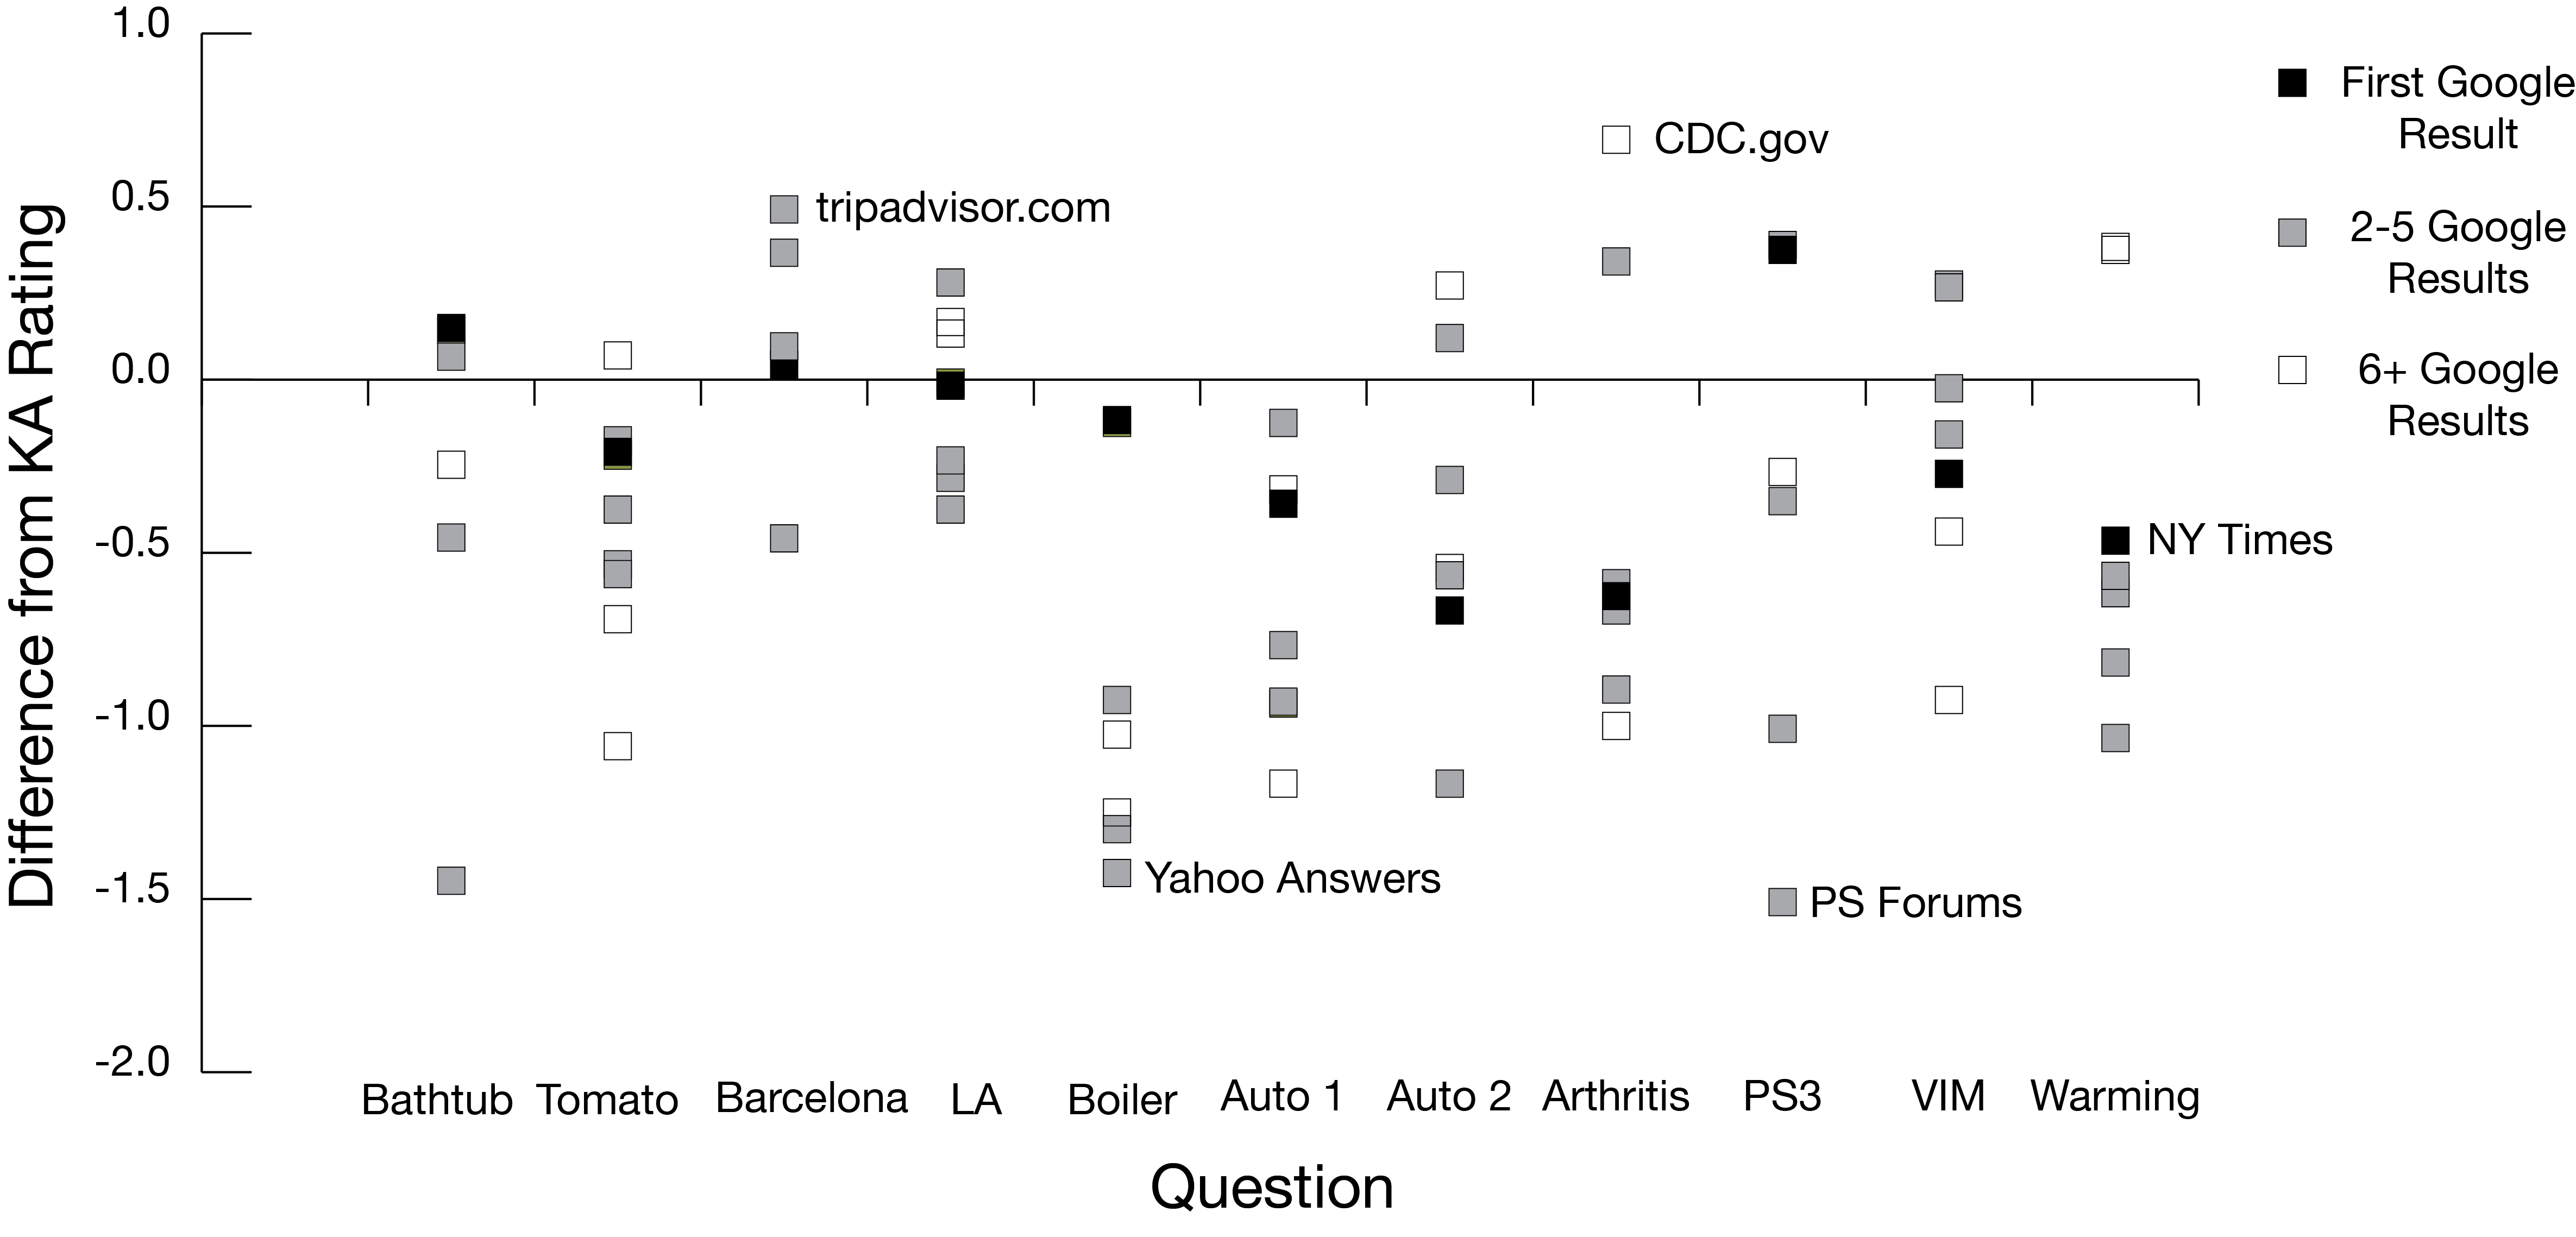
\includegraphics[width=1\columnwidth]{Chapters/KA/source_eval_graph}
    \caption[Results across questions and websites.]{Results across questions and websites. Points represent the average aggregate score difference between the KA answer and an existing site}
    \label{fig:aggregated}
\end{figure*}

\subsection{Results}
Aggregating across all questions, KA output was rated significantly higher than the comparison web pages, which included the top 5 Google results and sources cited more than 3 times (KA: $\bar{x} = 2.904$ vs Alt. Sites: $\bar{x} = 2.545$, $t(1493) = 13.062$, $p < 0.001$). An analysis of individual questions corrected for multiple comparisons is shown in Table~\ref{tab:evaluation}. 

The strongly positive results found were surprising because some of the websites in the comparison set were written by experts and had well-established reputations. Only on the two travel questions, Barcelona ($\bar{x} = -0.109$) and LA ($\bar{x} = -0.044$), and the VIM question ($\bar{x} = 0.180$) did the KA output not significantly outperform the comparison pages. A closer examination of these pages suggests that for the two travel questions, because of the strong internet commodity market surrounding travel, a considerable amount of effort has been spent on curating good travel resources. Even with the slightly more specific LA query, there were still two specialized sites dedicated to attraction for kids in LA (Mommypoppins.com and ScaryMommy.com). The VIM question represented a mismatch between our output and the question style. A number of the sources for the question were tutorials, however in the clipping phase, these ordered tutorials were broken up into unordered clips, creating an information model breakdown. This points out an interesting limitation in the KA approach, and suggests that adding support for more structured answers (e.g., including sequential steps) could be valuable future work. 

%\begin{figure}
%    \centering
%    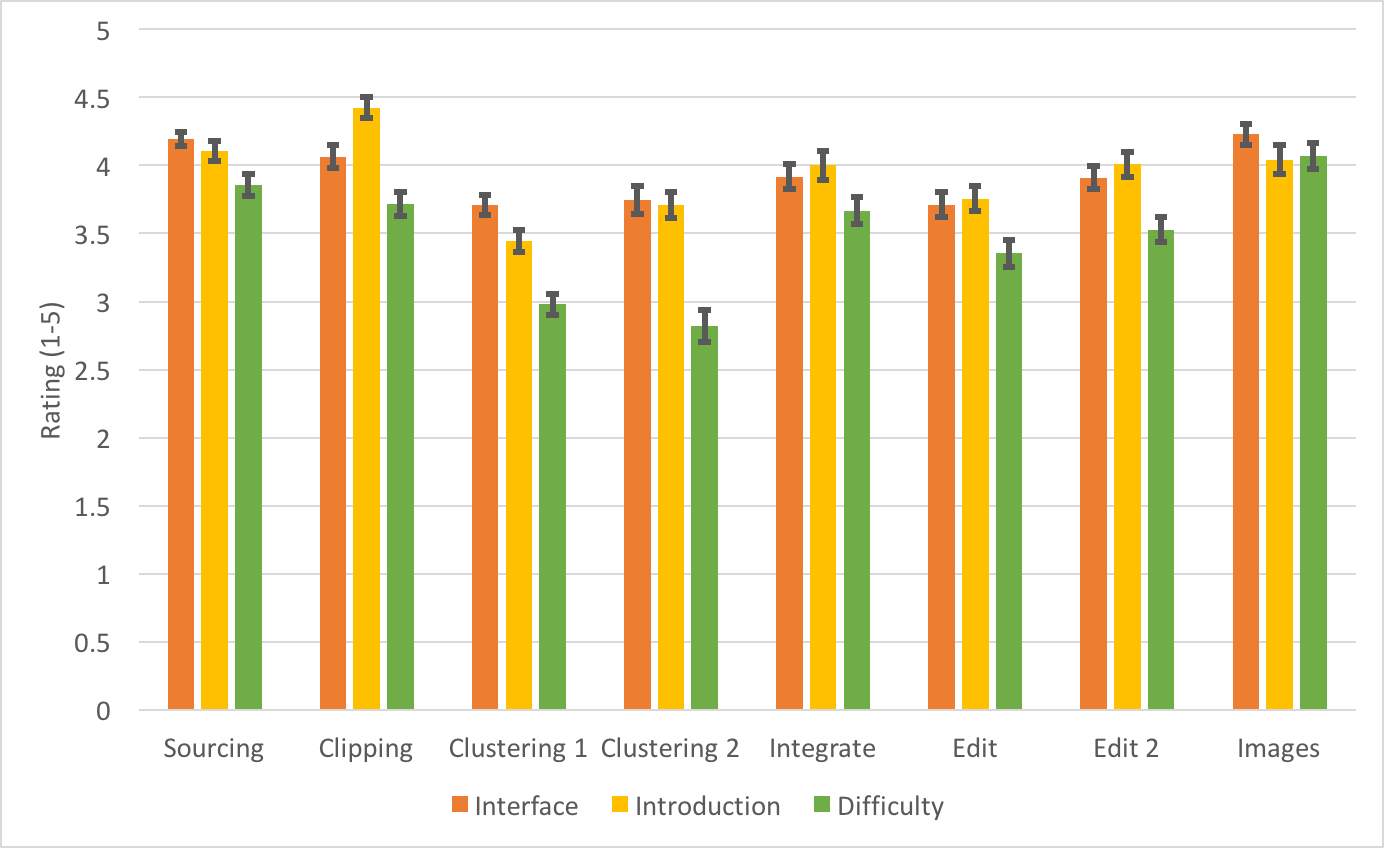
\includegraphics[width=1.0\columnwidth]{feedback}
%    \caption{Difficulty, instructions, and interface ease of use self-report from workers participating in the KA system. A lower number indicates a higher difficulty, poorer instructions, or a difficult interface.}
%    \label{fig:feedback}
%\end{figure}

As an additional external evaluation, for the two questions (Q6 and Q7) related to automotive systems we compared the discovered categories from the KA system with two commercial knowledge service products generated by expert technicians. We compared the KA response's accuracy and comprehensiveness, and found that it discovered all the categories referred to in these two commercial products for each question. Furthermore, the categories from the KA output provided more categories not mentioned in the commercial product (average 2.5 categories from two commercial products, while average 9.5 categories from KA). We validated these additional categories with expert automotive professionals who evaluated them as also being plausible and reasonable for the given questions. There was one instance in which two distinct categories (Encoder Motor and Encoder Motor Sensor) from the commercial products were clustered into the single category named Encoder Motor Assembly in the KA output. However, the full text answer from the KA system for Encoder Motor Assembly did still contain these two sub-components with different repair procedures. 

It may seem surprising that KA would work well for questions such as automotive error codes, where the response relies heavily on technical knowledge and jargon. On further inspection we believe this is because there are many online resources that have valuable information pertaining to these questions but are in unstructured and dialog oriented forms. Workers in the sourcing phase found rich sources of online information from many car enthusiast discussion forums, in which members tried to diagnose and help each other solve their automative problems. Although crowd workers may not understand the esoteric jargon of the automative domain, their understanding of grammar, semantics, and argument structure was sufficient to let them find, filter, cluster, integrate, and edit this domain-specific information. These results suggest a interesting avenue for future research leveraging human understanding of semantics and argument structure to extend crowdsourcing to process expert domain knowledge and to understand the limits of where such an approach breaks down.

%(see Figure~\ref{fig:feedback})

On average, running a question through the KA system cost a total of \$108.50 (see Table~\ref{tab:cost}). Although our primary goal was to establish a proof of concept of accomplish big picture thinking in small pieces, we return to the issue of cost in the Discussion. From the self-report crowdworker feedback, workers mostly found the tasks to be easy to complete, with the clustering phase having the most difficult task.

\begin{table}[ht]
  \centering
% question, number of sources, number of clips, number of turkers
  \begin{tabular}{lrrr}
    \hline
    \textbf{Phase} & \textbf{Task Pay} & \textbf{Avg. \# of Tasks} & \textbf{Avg. Cost} \\
    \hline
	Sourcing & \$0.25 & 15 & \$3.75 \\

    Clipping & \$0.50 & 21.6 & \$10.80 \\

    Clustering 1 & \$1.00 & 10 & \$10.00 \\

    Clustering 2 & \$1.00 & 10 & \$10.00 \\

    Integrate & \$0.50 & 37.2 & \$18.60 \\

    Edit 1 & \$0.75 & 28.8 & \$21.60 \\

    Edit 2 & \$1.00 & 28.8 & \$28.80 \\

    Images & \$0.50 & 9 & \$4.50 \\
    \hline    
    \textbf{Total} & & 160.4 & \$108.05 \\
    \hline
  \end{tabular}
  \caption[Average number of worker tasks and cost of running KA.]{Average number of worker tasks and average cost per phase, and overall, to run a question.}
  \label{tab:cost}
\end{table}
%The most notable result was the difference in output for different question types. Ideally, any question posed should be answerable by the system. However, the KA system appeared to do significantly better for some types of questions, while it was mediocre, or worse, for other types of questions. Therefore, we think the KA system is very effective for questions that fall on the "long tail" of search queries \cite{bernstein2012direct}. The output from the KA system, for any question, might be considered acceptable, and that acceptableness shines when the other available sources are poor or too general. Questions 5 through 10 show this, as those questions feature either a modifier to the query e.g Q8's "as a 28 year old" or are specific to a particular product (Q5-7, Q9). 

%Some of the qualitative feedback we received seemed to suggest this as well. For Q3, individuals noted that the message was often ``a lot better conveyed" than the KA output or the competing website was just ``simpler." For Q2 and Q4, raters noted the KA output just ``throws too much information at you" and also the layout made it difficult to read all of the content. However, for Q5-7, many of the raters noted that the sites appeared to be very "unprofessional" and the KA system "actually has useful information about the problem ... [alt website] is filled with questions without answers." 
\section{Discussion}

Our primary goal was to investigate the opportunities and limitations of accomplishing big thinking in small pieces, using a distributed information synthesis task as a probe. We instantiated our design approach in a prototype system called the Knowledge Accelerator which crowdsourced the process under the constraint that no single task would pay more than \$1, and investigated its performance across a variety of complex information seeking questions. Results suggested that the output of the system compared favorably to top information sources on the web, approaching or exceeding perceived quality ratings for even highly curated and reputable sources.

The strong performance of the system is perhaps surprising given that its output was generated by many non-expert crowd workers, none of whom saw the big picture of the whole. We do not believe that this should be interpreted as a replacement for expert creation and curation of content. Instead, the power of the system may actually be attributable to the value created by those experts by generating content which the crowd workers could synthesize and structure into a coherent digest. This explanation suggests that the approach would be most valuable where experts generate a lot of valuable information that is unstructured and redundant, such as the automative questions in which advice from car enthusiasts was spread across many unstructured discussion forums. In contrast, KA's output did not outperform top web sources for topics such as travel, where there are heavy incentives for experts to generate well structured content.  We believe its performance is likely due to its aggregation of multiple expert viewpoints rather than particularly excellent writing or structure per se, though this is a fruitful area for future investigation.

In developing the KA system, we explored a number of approaches that did not work. We initially tried to avoid a clustering phase altogether by exploring variations of the clipping task in which we provided additional context to workers in having them read through multiple sources, engage the workers who found sources in doing the clipping, or have them build on the categories that other workers had already generated rather than work independently.  However, in all cases workers did not generate good labels due to a lack of context. We then explored introducing an additional ``conductor'' view, in which workers could be recruited as clips came in to organize those clips and close categories that had a sufficient number of clips; however, this also failed because the conductors did not have sufficient global context to create good categories. These failures motivated the hybrid crowd-machine clustering phase.

Development of the integration and editing phases also included many false starts due to the opposite problem of giving workers \textit{too much} context. Our first integration interface enabled multiple workers at the same time to easily view and expand all the clips in a category for within-category context, and also see the current state of how other categories were developing for between-category context. Our idea was that as workers integrated clips and built out more options exposure to the other clips and options in real time would help them create more coherent digests. However, this approach proved overwhelming for scaling up to a large number of crowd workers engaged for short time periods. This motivated us to split up within-category and across-category consistency into the integration and editing phases and the development of the vote-edit pattern.

We encountered a number of places where our approach could be improved. As evidenced in the VIM question, the lack of support for nuanced structure in our digests can prove problematic. For some sources such as tutorials or how-tos, supporting sequential dependencies between steps could be useful. While our output was able to support such dependencies in an ad-hoc way within a category (such as the sequential steps for plunging a drain) it would be profitable to be able to support sequential dependencies across categories (e.g., first try x, then try y). More structure could also be beneficial for particular domain areas, such as explicitly capturing symptoms and causes as different types for automotive or medical diagnostic questions.

%Overall the KA system performed well, considering the number of existing curated sources. One of the most interesting results from the evaluation was the different performance for different questions. While initially we attributed this to the KA system only performing well for certain question types, in reality it had to do with the search results. If Google was able to return a large amount of high quality results, such as for a travel question, the KA output was not significantly better. This suggests that the KA system output is very good in most cases, but it's much harder to tell when comparing to other strong articles. This becomes especially apparent in the extremely specialized questions, such as the boiler or automotive questions. 

%While we tried to emulate the individual model of sensemaking, one of the biggest pieces, iteration, is severely lacking from our system. Sensemaking theories \cite{dervin1983overview, dervin1998sense,pirolli1999information,Russell:1993:CSS:169059.169209} agree there is this constant process of searching for information, and improving a mental model based on the gathered information. In online information foraging, this process can be observed in the form of querying a information retrieval engine, learning new knowledge from the search results, and reformulating the next query \cite{Gayo-Avello:2009:SSD:1523512.1523556,Spink:1998:MUS:865316,swanson1977information}. However, in our system, there is only one phase of searching and structuring. 

%We somewhat avoid this due to our delayed structuring design pattern. In individual sensemaking, this is iteration partially due to limitations of working memory and serial processing constraints, as each piece of information is costly in time and storage to consume. In contrast, distributing the information synthesis process across individuals and using computation to help store and cluster information relaxes these constraints significantly. Thus instead of iterating to find a better structure, KA instead casts a wider initial net (which can be done by many workers in parallel) to have better context when doing the structuring. 

The system could also benefit from including iteration. For example, after workers completed the integration phase they were asked the question ``What else needs to be done to make this a complete answer?''. While many obviously said the section needed be edited, one of the most popular responses was ``Needs more information.'' This suggested to us that while our clips and categories had pulled in most of the information, there was more information in some sections we were missing. One possibility is to introduce an iterative component at this point -- as workers are integrating information into the pad and notice missing information, they can request for other workers to go out and find that additional information through clipping. %Another possibility is to introduce iteration earlier during the clustering phase. Individuals could pose questions or missing content areas when reviewing the clusters, prompting a second round of sourcing and filtering for a more refined question.%
Thus while the system was partially successful at taking a breadth-oriented approach rather than the deeply iterative approach typical of sensemaking \cite{dervin1983overview, dervin1998sense,pirolli1999information,Russell:1993:CSS:169059.169209}, understanding how to best incorporate iteration would be a valuable area for future work.

A final area for future improvement is the cost associated with producing answers. Our digests took approximately \$100 to produce. While intended as a proof-of-concept prototype and similar in scale to other such crowdsourcing systems \cite{andre2014crowd,Chilton:2013:CCT:2470654.2466265}, it is interesting to consider what could be done to move the approach towards a useful production system with lowered costs. One area of improvement is optimization: by dynamically deciding how many workers and products to use in each stage final costs could be dropped significantly (e.g., as in \cite{Kamar:2012:CHM:2343576.2343643}). Furthermore, for many practical information seeking purposes the categories and associated clips may be sufficent, which would obviate the need for the expensive stages of integration and editing and reduce costs by over 65\%. 

Perhaps the most interesting possibility is if answers could be reused across questions. Although users have complex information seeking needs, many of the queries they issue are similar. For example, a recent study estimated that 3\% of search queries account for one third of total search volume \cite{white2007studying}. Thus at a minimum, many answers could be amortized across users with the same question. A particularly promising but challenging opportunity is if similar questions may be able to reuse components of already summarized answers; for example, a question on investing advice for a 50 year old might use some common categories as for a 20 year old, but others would be unique to the new question's context. Challenges for the reuse of information are how the system would be able to identify the similarity for possible answers during each information synthesis phase and what level of granularity should be considered to for an effective system. Spatial and temporal reasoning over the existing knowledge and new information could be considered to provide context-aware and up-to-date answers. 

We hope the design choices embodied in the KA prototype system and the design patterns discussed here may be useful for other system designers working to distribute cognitive complex tasks. Some domains that might benefit from this include microtask markets, which could benefit from supporting more complex tasks; volunteer crowdsourcing efforts such as Wikipedia \cite{kittur2008harnessing} or friendsourcing in which many small contributions are readily available \cite{bernstein2010personalization}; or self-sourcing in which the crowd within could accomplish complex tasks in small increments (e.g., waiting for the bus) without needing to load the entire task context into working memory \cite{teevan2014selfsourcing}. Overall, we believe this approach represents a step towards a future of big thinking in small packages, in which complex and interdependent cognitive processes can be scaled beyond individual cognitive limitations by distributing them across many individuals.

%\section{Acknowledgments}

%The authors would like to thank to Andrew Peters for his initial work on the KA system. This work was supported by NSF grants IIS-1149797, IIS-0968484, IIS-1111124, Bosch, and Google.

%\section{Appendix}

%See \url{http://nhahn.org/portfolio/ka.html\#appendix} for additional resources, including the original articles generated by the KA system.

% Balancing columns in a ref list is a bit of a pain because you
% either use a hack like flushend or balance, or manually insert
% a column break.  http://www.tex.ac.uk/cgi-bin/texfaq2html?label=balance
% multicols doesn't work because we're already in two-column mode,
% and flushend isn't awesome, so I choose balance.  See this
% for more info: http://cs.brown.edu/system/software/latex/doc/balance.pdf
%
% Note that in a perfect world balance wants to be in the first
% column of the last page.
%
% If balance doesn't work for you, you can remove that and
% hard-code a column break into the bbl file right before you
% submit:
%
% http://stackoverflow.com/questions/2149854/how-to-manually-equalize-columns-
% in-an-ieee-paper-if-using-bibtex
%
% Or, just remove \balance and give up on balancing the last page.
%
